\documentclass{article}
\usepackage[sexy, hdr, fancy]{evan}
\setlength{\droptitle}{-4em}

\lhead{Homework 9}
\rhead{Introduction to Statistics}
\lfoot{}
\cfoot{\thepage}

\newcommand{\var}{\mathrm{Var}}
\newcommand{\cov}{\mathrm{Cov}}

\begin{document}
\title{Homework 9}
\maketitle
\thispagestyle{fancy}

\section*{Chapter 12: The Analysis of Variance}

\begin{itemize}
	\item[5.] Derive the likelihood ratio for the null hypothesis of the one-way layout, and show that it is equivalent to the $F$ test in the case $I=2.$
		\begin{proof}
			In the case $I=2,$ we have two treatments. Suppose that $X_i$ and $Y_i$ are data from the two treatments, and there are $J$ observations for each. We have $H_0:\mu_X=\mu_Y=\mu_0.$ Assuming $X_i$ and $Y_i$ are normal variables with common variance $\sigma^2,$ the numerator of the likelihood ratio is evaluated at the value of $\mu_0$ that maximizes the likelihood function
			\[f(X_i, Y_i\mid \mu_0) = \prod_{i=1}^{J} \frac{1}{\sigma\sqrt{2\pi}}\exp\left( -\frac{(X_i-\mu_0)^2}{2\sigma^2} \right)\prod_{i=1}^{J} \frac{1}{\sigma\sqrt{2\pi}}\exp\left( -\frac{(Y_i-\mu_0)^2}{2\sigma^2} \right)\]
			which is $\mu_0=\frac{\bar X + \bar Y}{2}.$
			
			The denominator of the likelihood ratio is the likelihood function using $\mu_X$ and $\mu_Y$ at the MLE, which are $\bar X$ and $\bar Y,$ respectively. Thus, the denominator is 
			\[f(X_i, Y_i) = \prod_{i=1}^{J}\frac{1}{\sigma\sqrt{2\pi}}\exp\left( -\frac{(X_i-\bar X)^2}{2\sigma^2} \right)\prod_{i=1}^{J}\frac{1}{\sigma\sqrt{2\pi}}\exp\left( -\frac{(Y_i-\bar Y)^2}{2\sigma^2} \right)\]

			The constants cancel in the ratio, and we are left with 
			\[\exp\left( -\frac{1}{2\sigma^2}\left[ \left( \sum_{i=1}^{J}(X_i-\mu_0)^2 + \sum_{i=1}^{J}(Y_i-\mu_0)^2 \right) - \left( \sum_{i=1}^{J}(X_i-\bar X)^2 + \sum_{i=1}^{J}(Y_i-\bar Y)^2 \right) \right] \right)\]
			Using $\mu_0=\frac{\bar X+\bar Y}{2}$ and some algebra, this simplifies to
			\[\Lambda = \exp\left( -\frac{J}{4\sigma^2}(\bar X-\bar Y)^2 \right)\]

			The $F$ test statistic in the case $I=2$ is
			\[F=\frac{SS_B/(I-1)}{SS_W/[I(J-1)]} = \frac{SS_B}{SS_W/[2(J-1)]}\]
			Here, the grand mean is given by $\frac{\bar X+\bar Y}{2}.$ Thus, we have
			\begin{align*}
				SS_B &= J\left[\left( \bar X- \frac{\bar X + \bar Y}{2}\right)^2 + \left( \bar Y-\frac{\bar X+\bar Y}{2} \right)^2\right] \\
				&= 2J\left( \frac{\bar X - \bar Y}{2} \right)^2 = \frac{J}{2}(\bar X-\bar Y)^2
			\end{align*}
			Then
			\begin{align*}
				\frac{SS_W}{2(J-1)} &= \frac{1}{2(J-1)}\left(\sum_{i=1}^{J}(X_i-\bar X)^2 + \sum_{i=1}^{J} (Y_i-\bar Y)^2 \right) = s_p^2
			\end{align*}
			so the $F$ test is given by
			\[F=\frac{J}{2\sigma_p^2}(\bar X-\bar Y)^2\]
			and the null hypothesis is rejected if $F$ is large. If $F$ is large, then $\exp(-F/2)$ is small, which is the same condition for rejecting the null hypothesis using the likelihood ratio.
		\end{proof}

	\item[7.] Show that, as claimed in Theorem B of Section 12.2.1, $SS_B/\sigma^2\sim\chi_{I-1}^2.$
		\begin{proof}
			We have
			\begin{align*}
				SS_B&=J\sum_{i=1}^{I}(\bar Y_{i\cdot} - \bar Y_{\cdot\cdot})^2 \\
				\implies \frac{SS_B}{\sigma^2} &= \sum_{i=1}^{I}\frac{(\bar Y_{i\cdot}-\bar Y_{\cdot\cdot})^2}{\sigma^2/J}
			\end{align*}	
			We know that $\var(\bar Y_{i\cdot}) = \sigma^2/J$ since it is a sample mean, and
			\begin{align*}
				s^2&=\frac{1}{I-1} \sum_{i=1}^{I}(\bar Y_{i\cdot}-\bar Y_{\cdot\cdot})^2 \\
				\implies \frac{(I-1)s^2}{\sigma^2/J} &= \sum_{i=1}^{J}\frac{(\bar Y_{i\cdot}-\bar Y_{\cdot\cdot})^2}{\sigma^2/J} = \frac{SS_B}{\sigma^2}
			\end{align*}
			which by Theorem B of Section 6.3 follows a $\chi_{I-1}^2$ distribution, as desired.
		\end{proof}

	\item[11.] Consider a hypothetical two-way layout with four factors (A, B, C, D) each at three levels (I, II, III). Construct a table of cell means for which there is no interaction.
		\begin{soln}
			The following table shows no interactions:
			\begin{center}
				\begin{tabular}{c|cccc}
					& A & B & C & D \\
					\hline
					I & 1 & 2 & 3 & 4 \\
					II & 5 & 6 & 7 & 8\\
					III & 9 & 10 & 11 & 12
				\end{tabular}
			\end{center}
		\end{soln}

	\item[12.] Consider a hypothetical two-way layout with three factors (A, B, C) each at two levels (I, II). Is it possible for there to be interactions but no main effects?
		\begin{answer*}
			Yes, this is possible. The means may be the same, but they could still cross over.
		\end{answer*}

	\item[21.] Use both graphical techniques and the $F$ test to test whether there are significant differences among the four groups. 
		\begin{soln}
			In R, the $F$ test had a value of 2.271 and a $p$-value of 0.115, so at the level $\alpha=0.05$ we conclude that there are no main effects.
		\end{soln}

	\item[34.] Conduct a two-way analysis of variance to test the effects of the two main factors and their interaction.
		\begin{soln}
			In R, the $F$ test for difference in treatments had value 14.015 and $p$-value $3.28\times 10^{-6}$ so the treatments differ. The $F$ test for difference in poisons had value 23.570 and $p$ value $2.86\times 10^{-7}$ so the poisons differ. The $F$ test for interactions had value 1.887 and $p$-value 0.11. If we are at a significance level $\alpha=0.05,$ then the interactions are not significant.

			Conducting Tukey's test for treatments at the significance level $\alpha=0.05,$ we conclude that the means differ between the pairs of treatments (A, B), (A, C), (B, D).

			Conducting Tukey's test for poisons at the significance level $\alpha=0.05,$ we conclude that the means differ between the pairs of poisons (1, 3), (2, 3).
		\end{soln}

\end{itemize}

\section*{Chapter 14: Linear Least Squares}

\begin{itemize}
	\item[1.] Convert the following relationships into linear relationships by making transformations and defining new variables.
		\begin{enumerate}[a.]
			\item $y=a/(b+cx)$
				\begin{soln}
					Let $z=1/y.$ Then \[\frac{1}{z} = \frac{a}{b+cx} \implies z = \frac{b}{a} + \frac{c}{a}x\] which is a linear relation.
				\end{soln}

			\item $y=ae^{-bx}$
				\begin{soln}
					Let $z=\log y.$ Taking the log of both sides, we have \[\log y = z = \log a - bx\] which is a linear relation.
				\end{soln}

			\item $y=ab^x$
				\begin{soln}
					Let $z=\log y.$ Taking the log of both sides, we have \[\log y = z = \log a+x\log b\] which is a linear relation.
				\end{soln}

			\item $y=x/(a+bx)$
				\begin{soln}
					Let $w=1/x$ and $z=1/y.$ Then we have \[\frac{1}{y} = z = \frac{a}{x} + b = aw + b\] which is a linear relation.
				\end{soln}

			\item $y=1/(1+e^{bx})$
				\begin{soln}
					Let $z=\log\left( \frac{1}{y} - 1 \right).$ Then we have \[\frac{1}{y} - 1 = e^{bx} \implies \log \left( \frac{1}{y} - 1 \right) = z = bx\] which is a linear relation.
				\end{soln}
				
		\end{enumerate}

	\item[2.] Plot $y$ versus $x:$
		\begin{enumerate}[a.]
			\item Fit a line $y=a+bx$ by the method of least squares, and sketch it on the plot.
				\begin{center}
					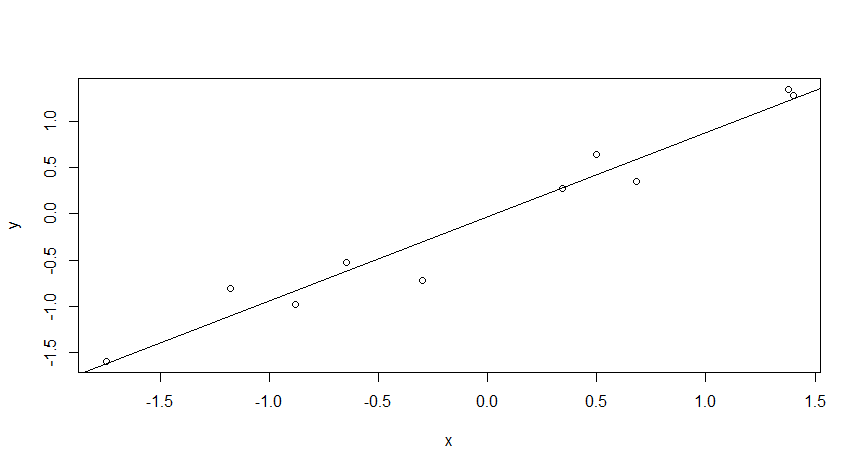
\includegraphics[width=14cm]{reg_x.png}
				\end{center}
				
			\item Fit a line $x=c+dy$ by the method of least squares, and sketch it on the plot.
				\begin{center}
					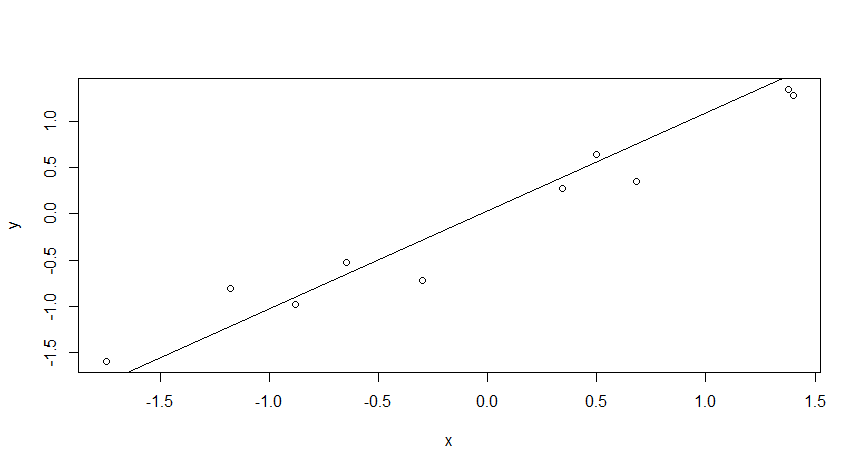
\includegraphics[width=14cm]{reg_y.png}
				\end{center}	

			\item Are the lines in parts (a) and (b) the same? If not, why not?
				\begin{answer*}
					They are not the same line. $y=a+bx$ minimizes least squares with the $y$ values, while $x=c+dy$ minimizes least squares with the $x$ values.
				\end{answer*}

		\end{enumerate}

		\newpage
	\item[3.] Suppose that $y_i=\mu+e_i,$ where $e_i$ are independent errors with mean zero and variance $\sigma^2.$ Show that $\bar y$ is the least squares estimate of $\mu.$
		\begin{proof}
			Let $\hat y$ be the least squares estimate of $\mu,$ which minimizes \[\sum_{i=1}^{n} (y_i-\hat y)^2 = \sum_{i=1}^{n} (\mu+e_i-\hat y)^2\] Taking the derivative with respect to $\hat y,$ we have
			\begin{align*}
				\frac{\partial}{\partial\hat y}\sum_{i=1}^{n} (\mu+e_i-\hat y)^2 &= -2\sum_{i=1}^{n} (\mu+e_i-\hat y) = 0 \\ 
				\implies n\mu-n\hat y + \sum_{i=1}^{n} e_i &= 0 \\
			\end{align*}
			Solving for $\hat y$ we obtain \[\hat y = \mu + \frac{1}{n} \sum_{i=1}^{n} e_i = \frac{1}{n} \sum_{i=1}^{n} (\mu+e_i) = \bar y\] as desired.
		\end{proof}

	\item[6.] Two objects of unknown weights $w_1$ and $w_2$ are weighed on an error-prone pan balance in the following way: (1) object 1 is weighed by itself, and the measurement is 3g; (2) object 2 is weighed by itself, and the result is 3g; (3) the difference of the weights (1-2) is 1g; (4) the sum of the weights measured as 7g. The problem is to estimate the true weights of the objects from these measurements.
		\begin{enumerate}[a.]
			\item Set up a linear model, $\mathbf{Y}=\mathbf{X}\mathbf{\beta}+\mathbf{e}.$
				\begin{soln}
					We have the system
					\begin{align*}
						w_1 + e_1 &= 3 \\
						w_2 + e_2 &= 3 \\
						w_1-w_2+e_3 &= 1 \\
						w_1+w_2+e_4 &= 7
					\end{align*}
					which corresponds to the equation 
					\[\begin{bmatrix}
							3 \\ 3 \\ 1 \\ 7
						\end{bmatrix} = \begin{bmatrix}
							1 & 0 \\ 0 & 1 \\ 1 & -1 \\ 1 & 1
						\end{bmatrix}\begin{bmatrix}
							w_1 \\ w_2
						\end{bmatrix} + \begin{bmatrix}
							e_1 \\ e_2 \\ e_3 \\ e_4
					\end{bmatrix}\]
				\end{soln}

			\item Find the least squares estimates of $w_1$ and $w_2.$
				\begin{soln}
					Let $\hat w_1$ and $\hat w_2$ be the least squares estimates of $w_1$ and $w_2,$ respectively. Then the sum of squares is given by
					\[(3-\hat w_1)^2 + (3-\hat w_2)^2 + (1-\hat w_1+\hat w_2)^2 + (7-\hat w_1-\hat w_2)^2\]
					Taking the derivatives with respect to $\hat w_1$ and $\hat w_2,$ we get
					\begin{align*}
						-2(3-\hat w_1) - 2(1-\hat w_1 + \hat w_2) - 2(7-\hat w_1-\hat w_2) &= 0 \implies \hat w_1 = \frac{11}{3} \\
						-2(3-\hat w_2) + 2(1-\hat w_1 + \hat w_2) - 2(7-\hat w_1-\hat w_2) &= 0 \implies \hat w_2 = 3
					\end{align*}
					as the least squares estimates.
				\end{soln}

			\item Find the estimate of $\sigma^2.$
				\begin{soln}
					With the two estimates above, we have
					\[\begin{bmatrix}
							e_1 \\ e_2 \\ e_3 \\ e_4
						\end{bmatrix} = \begin{bmatrix}
							-2/3 \\ 0 \\ 1/3 \\ 1/3
					\end{bmatrix}\]
					We know that $e_i$ are iid with variance $\sigma^2,$ so we calculate the sample variance $s^2$ to estimate $\sigma^2,$ which is $2/9.$
				\end{soln}

			\item Find the estimated standard errors of the least square estimates of part (b).
				\begin{soln}
					We have $(\mathbf{X}^T \mathbf{X})\inv=\left( \begin{bmatrix}
						3 & 0 \\ 0 & 3
					\end{bmatrix}\right)\inv = \begin{bmatrix}
						1/3 & 0 \\ 0 & 1/3
					\end{bmatrix}.$ Thus, the estimated standard errors are 
					\[s_{\hat w_1} = s\sqrt{1/3} = \sqrt{2/9}\sqrt{1/3} = \sqrt{2/27} = s_{\hat w_2}\]
				\end{soln}

			\item Estimate $w_1-w_2$ and its standard error.
				\begin{soln}
					We estimate with 
					\[\hat w_1-\hat w_2 = \frac{11}{3} - 3 = \frac{2}{3}\]
					Next,
					\begin{align*}
						\var(\hat w_1-\hat w_2) &= \var(\hat w_1)+\var(\hat w_2) - 2\cov(\hat w_1, \hat w_2) \\
						&= 2\cdot\frac{2}{27} - 2*0 = \frac{4}{27}
					\end{align*}
					so the standard error is
					\[s_{\hat w_1-\hat w_2} = \frac{2}{3\sqrt{3}}\]
				\end{soln}

			\item Test the null hypothesis $H_0: w_1=w_2.$
				\begin{soln}
					We use the test statistic
					\[\frac{\hat w_1-\hat w_2}{s_{\hat w_1-\hat w_2}} = \frac{2/3}{2/(3\sqrt{3})} = \sqrt{3}\]
					which is a $t$ distribution with 3 degrees of freedom. The $p$ value associated with this is 0.0908. At the significance level $\alpha=0.1,$ we would reject the null hypothesis that $w_1=w_2.$
				\end{soln}
				
		\end{enumerate}

		\newpage
	\item[10.] Show that the least squares estimate of the slope and intercept of a line may be expressed as \[\hat\beta_0=\bar y-\hat\beta_1\bar x\] and \[\hat\beta_1=\frac{\displaystyle \sum_{i=1}^{n} (x_i-\bar x)(y_i-\bar y)}{\displaystyle \sum_{i=1}^{n} (x_i-\bar x)^2}\]
		\begin{proof}
			Let $y=\hat\beta_0 + \hat\beta_1x$ be the least squares line. Thus, the sum of squares
			\[\sum_{i=1}^{n}(y_i - \hat\beta_0-\hat\beta_1x_i)^2\]
			is minimized. Taking the derivative with respect to $\hat\beta_0,$ we have 
			\begin{align*}
				-2\sum_{i=1}^{n} (y_i-\hat\beta_0-\hat\beta_1) &= -2\left( \sum_{i=1}^{n} y_i -n\hat\beta_0 - \hat\beta_1\sum_{i=1}^{n} x_i \right) = 0 \\
				\implies n\bar y - n\hat\beta_0 - n\hat\beta_1 \bar x &= 0 \\
				\implies \hat\beta_0 &= \bar y - \hat\beta_1\bar x
			\end{align*}
			as desired.

			Next, taking the derivative with respect to $\hat\beta_1,$ we have
			\begin{align*}
				-2\sum_{i=1}^{n}x_i(y_i-\hat\beta_0-\hat\beta_1 x_i) &= -2\left( \sum_{i=1}^{n} x_iy_i - \hat\beta_0 \sum_{i=1}^{n} x_i - \hat\beta_1\sum_{i=1}^{n} x_i^2 \right) = 0 \\
				\implies \sum_{i=1}^{n} x_iy_i - (\bar y - \hat\beta_1\bar x)\sum_{i=1}^{n} x_i - \hat\beta_1 \sum_{i=1}^{n}x_i^2 &= 0 \\
				\implies \sum_{i=1}^{n} x_iy_i - n\bar x\bar y + n\hat\beta_1\bar x^2 - \hat\beta_1 \sum_{i=1}^{n} x_i^2 &= 0 \\
				\implies \hat\beta_1 \left(\sum_{i=1}^{n} x_i^2 -n\bar x^2\right) &= \sum_{i=1}^{n} x_iy_i-n\bar x\bar y
			\end{align*}
			We have
			\begin{align*}
				\sum_{i=1}^{n} (x_i-\bar x)^2 &= \sum_{i=1}^{n} x_i^2 - \bar x\sum_{i=1}^{n} x_i + n\bar x^2 \\
				&= \sum_{i=1}^{n} x_i^2 - n\bar x^2 \\
				\sum_{i=1}^{n} (x_i-\bar x)(y_i-\bar y) &= \sum_{i=1}^{n} x_iy_i - \bar x\sum_{i=1}^{n} y_i - \bar y\sum_{i=1}^{n} x_i + n\bar x\bar y \\
				&= \sum_{i=1}^{n} x_iy_i - n\bar x\bar y - n\bar x\bar y + n\bar x\bar y = \sum_{i=1}^{n} x_iy_i - n\bar x\bar y
			\end{align*}
			Thus, solving for $\hat\beta_1,$ we have 
			\[\hat\beta_1 = \frac{\displaystyle\sum_{i=1}^{n} x_iy_i-n\bar x\bar y}{\displaystyle\sum_{i=1}^{n} x_i^2 - n\bar x^2} = \frac{\displaystyle\sum_{i=1}^{n} (x_i-\bar x)(y_i-\bar y)}{\displaystyle\sum_{i=1}^{n} (x_i-\bar x)^2}\]
			as desired.
		\end{proof}

	\item[11.] Show that if $\bar x=0,$ the estimated slope and intercept are uncorrelated under the assumptions of the standard statistical model.
		\begin{proof}
			The covariance of $\hat\beta_0$ and $\hat\beta_1$ are given by
			\begin{align*}
				\cov(\hat\beta_0, \hat\beta_1) &= \frac{-\displaystyle\sigma^2\sum_{i=1}^{n} x_i}{\displaystyle n\sum_{i=1}^{n} x_i^2-\left( \sum_{i=1}^{n} x_i \right)^2}
			\end{align*}
			from Theorem B Section 14.2.1. If $\bar x=0,$ then the numerator is 0, so the covariance between the slope and intercept is 0, thus they are uncorrelated, as desired.	
		\end{proof}

	\item[12.] Use the result of Problem 10 to show that the line fit by the method of least squares passes through the point $(\bar x, \bar y).$
		\begin{proof}
			The least squares line is given by $y=\hat\beta_0+\hat\beta_1x.$ From Problem 10, we know that $\hat\beta_0=\bar y-\hat\beta_1\bar x,$ so $\bar y=\hat\beta_0+\hat\beta_1\bar x.$ Thus, the pair $(\bar x, \bar y)$ passes through the least squares line, as desired.
		\end{proof}

	\item[13.] Suppose that a line is fit by the method of least squares to $n$ points, that the standard statistical model holds, and that we want to estimate the line at a new point, $x_0.$ Denoting the value on the line by $\mu_0,$ the estimate is \[\hat\mu_0=\hat\beta_0+\hat\beta_1x_0\] 
		\begin{enumerate}[a.]
			\item Derive an expression for the variance of $\hat\mu_0.$
				\begin{soln}
					We have
					\begin{align*}
						\var(\hat\mu_0) &= \var(\hat\beta_0 + \hat\beta_1x_0) \\
						&= \var(\hat\beta_0) + x_0^2\var(\hat\beta_1)+2x_0\cov(\hat\beta_0, \hat\beta_1) \\
						&= \frac{\sigma^2\sum_{}^{}x_i^2}{n\sum_{}^{}x_i^2-\left( \sum_{}^{}x_i \right)^2} + x_0^2\frac{n\sigma^2}{n\sum_{}^{}x_i^2 - \left( \sum_{}^{}x_i \right)^2} + 2x_0\frac{-\sigma^2\sum_{}^{}x_i}{n\sum_{}^{}x_i^2-\left( \sum_{}^{}x_i \right)^2} \\
						&= \frac{\sigma^2}{n\sum_{}^{}x_i^2 - \left( \sum_{}^{}x_i \right)^2}\left(  \sum_{}^{}x_i^2 + nx_0^2 - 2x_0\sum_{}^{}x_i \right) \\
						&= \frac{\sigma^2}{n\sum_{}^{}(x_i-\bar x)^2}\sum_{}^{}\left(x_i^2+x_0^2-2x_0x_i \right) \\
						&= \frac{\sigma^2}{n} \cdot \frac{\sum_{}^{}(x_i-x_0)^2}{\sum_{}^{}(x_i-\bar x)^2} = \frac{\sigma^2}{n} \frac{\sum_{}^{}(x_i-\bar x+\bar x-x_0)^2}{\sum_{}^{}(x_i-\bar x)^2} \\
						&= \frac{\sigma^2}{n} \cdot \frac{\sum_{}^{}(x_i-\bar x)^2 + n(\bar x-x_0)^2 + 2(x_0-\bar x)\sum_{}^{}(x_i-\bar x)}{\sum_{}^{}(x_i-\bar x)^2} \\
						&= \frac{\sigma^2}{n} \left( 1+\frac{n(x_0-\bar x)^2}{\sum_{}^{}(x_i-\bar x)^2} \right) = \sigma^2\left( \frac{1}{n} + \frac{(x_0-\bar x)^2}{\sum_{}^{}(x_i-\bar x)^2} \right)
					\end{align*}
				\end{soln}

			\item Sketch the SD of $\hat\mu_0$ as a function of $x_0-\bar x.$ The slope of the curve should be intuitively plausible.
				\begin{answer*}
					As you can see above, my expression for the SD is a function of $x_0-\bar x.$ I'm not really sure how to go about sketching this without any sort of numbers.
				\end{answer*}

			\item Derive a 95\% confidence interval for $\mu_0=\beta_0+\beta_1x_0$ under an assumption of normality.
				\begin{soln}
					Under an assumption of normality, it holds that $\hat\mu_0$ follows a $t_{n-1}$ distribution and variance as found in part a. Using $s^2$ to estimate $\sigma^2,$ we have the 95\% confidence interval is given by
					\[(\beta_0+\beta_1x_0) \pm s\sqrt{\frac{1}{n} + \frac{(x_0-\bar x)^2}{\sum_{}^{}(x_i-\bar x)^2}} t_{n-2}(5/2)\]
				\end{soln}
				
		\end{enumerate}
			
	\item[14.] Problem 13 dealt with how to form a CI for the value of a line of at a point $x_0.$ Suppose that instead we want to predict the value of a new observation, $Y_0,$ at $x_0,$ \[Y_0=\beta_0+\beta_1x_0+e_0\] by the estimate \[\hat Y_0=\hat\beta_0+\hat\beta_1x_0\]
		\begin{enumerate}[a.]
			\item Find an expression for the variance of $\hat Y_0-Y_0,$ and compare it to the expression for the variance of $\hat\mu_0$ obtained in part (a) of Problem 13. Assume that $e_0$ is independent of the original observations and has the variance $\sigma^2.$
				\begin{soln}
					We have
					\begin{align*}
						\var(\hat Y_0-Y_0) &= \var(\hat Y_0) +\var(Y_0) - 2\cov(\hat Y_0, Y_0) \\
						&=\var(\hat\beta_0+\hat\beta_1 x_0) + \sigma^2 \\
						&= \sigma^2 \left( \frac{n+1}{n} + \frac{(x_0-\bar x)^2}{\sum_{}^{}(x_i-\bar x)^2}\right)
					\end{align*}
					since $\beta_0, \beta_1, x_0$ are all constants, and $e_0$ is independent from all of the original observations.
				\end{soln}

			\item Assuming that $e_0$ is normally distributed, find the distribution of $\hat Y_0-Y_0.$ Use this result to find an interval $I$ such that $P(Y_0\in I)=1-\alpha.$ This interval is called a $100(1-\alpha)\%$ prediction interval.
				\begin{soln}
					We have \[\hat Y_0-Y_0=(\hat\beta_0-\beta_0) + x_0(\hat\beta_1-\beta_1)-e_0\] which is a linear combination of normal random variables, so the distribution of $\hat Y_0-Y_0$ is normal with mean 0 and variance as given above. Thus, using $z_{\alpha/2}$ we can construct an interval around 0, and by adding $Y_0,$ we can construct an interval about $Y_0.$
				\end{soln}
				
		\end{enumerate}
		
		\newpage
	\item[40.] The following data come from the calibration of a proving ring, a device for measuring force.
		\begin{enumerate}[a.]
			\item Plot load versus deflection. Does the plot look linear?
				\begin{center}
					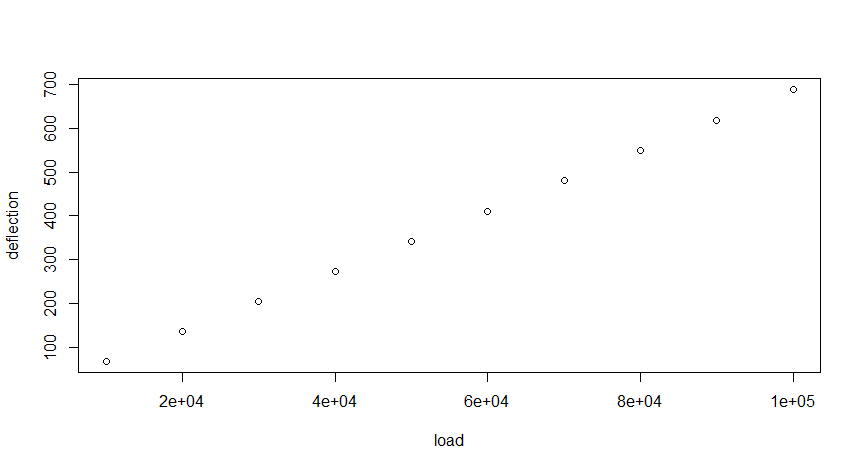
\includegraphics[width=14cm]{run_deflection.png}
				\end{center}
				\begin{answer*}
					The plot does look linear.
				\end{answer*}

			\item Fit deflection as a linear function of load, and plot the residuals versus load. Do the residuals show any systematic lack of fit?
				\begin{center}
					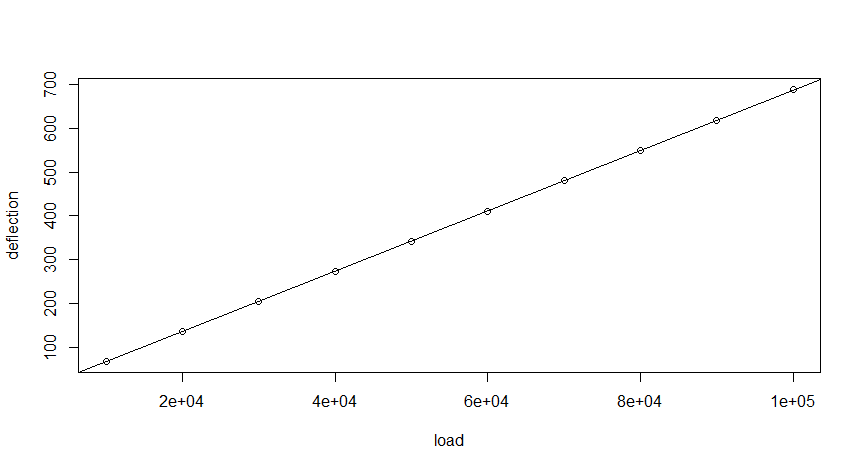
\includegraphics[width=14cm]{reg_load_def.png}
				\end{center}
				\begin{center}
					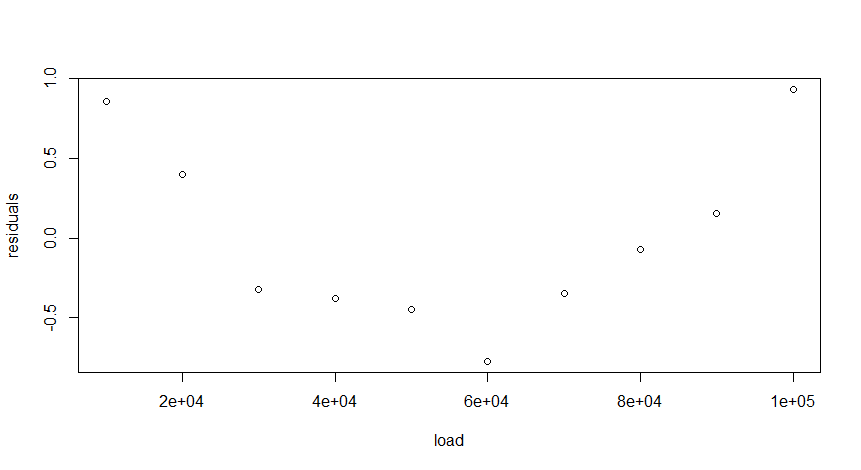
\includegraphics[width=14cm]{load_resid.png}
				\end{center}
				\begin{answer*}
					The residuals do not show a systematic lack of fit.
				\end{answer*}

		\end{enumerate}

\end{itemize}

\end{document}
